\chapter{補足}

\section{モンキーハンティング} \label{モンキーハンティング}

以下のような形式の問題を総称してモンキーハンティングと呼ぶ。

\begin{quote}
小球を、位置 $(0, 0)$ から初速 $v_0$、 仰角 $\theta$ で発射したところ、位置 $(l, h)$ から自由落下してくる物体に衝突した。 $\tan \theta$ の満たすべき条件を求めよ。ただし、重力加速度の大きさを $g$ とする。
\end{quote}

\begin{figure}[htb]
\centering
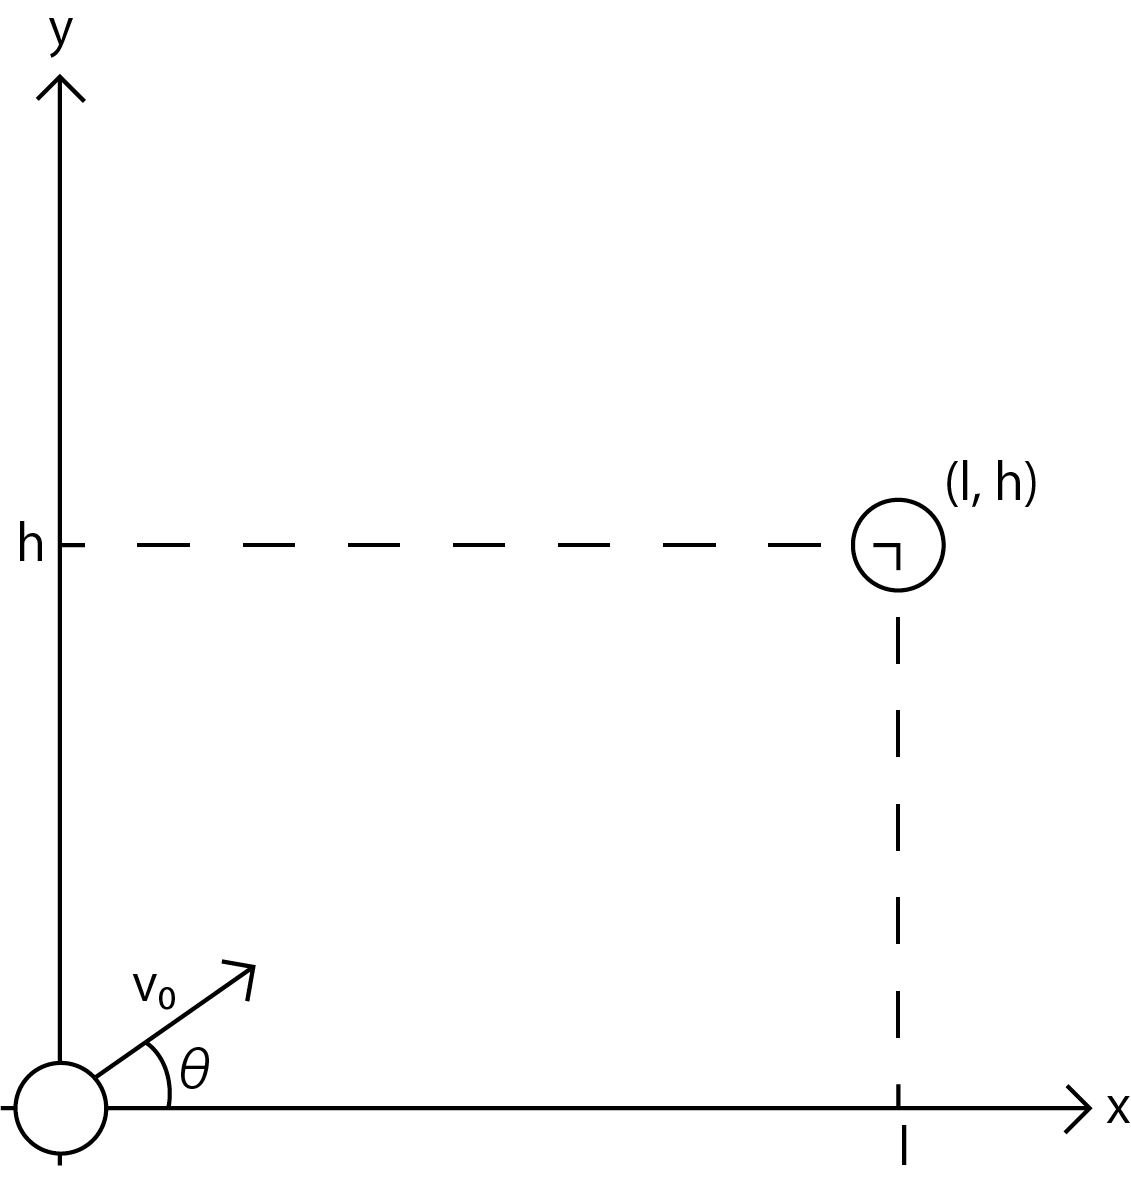
\includegraphics{work/monkey_hunting.png}
\end{figure}
